\subsection*{Problema 20}

\textbf{Enunciado:}
Calcular la integral:
\begin{align*}
\int \dfrac{x^4 - x^3 - 2x^2 - x + 2}{(x - 1)(x^2 + 2)^2} \, dx
\end{align*}

\textbf{Solución:}
El integrando es una función racional propia. 
Aplicamos fracciones parciales con un 
factor cuadrático repetido:
\begin{align*}
\dfrac{x^4 - x^3 - 2x^2 - x + 2}{(x - 1)(x^2 + 2)^2} &= 
\dfrac{A}{x - 1} \\
&+ \dfrac{Bx + C}{x^2 + 2} \\
&+ \dfrac{Dx + E}{(x^2 + 2)^2}
\end{align*}

Multiplicando por el denominador común 
$(x - 1)(x^2 + 2)^2$ y agrupando términos, 
obtenemos los coeficientes:
\begin{align*}
A &= 0, \quad B = 1, \quad C = 0, \\
D &= -1, \quad E = -1
\end{align*}

Sustituyendo los coeficientes:
\begin{align*}
\int &\dfrac{x}{(x^2 + 2)} \, dx \\
&- \int \dfrac{x + 1}{(x^2 + 2)^2} \, dx
\end{align*}

Para la primera integral, usamos sustitución 
simple $u = x^2 + 2$, $du = 2x \, dx$:
\begin{align*}
\int \dfrac{x}{x^2 + 2} \, dx &= \dfrac{1}{2}\ln|x^2 + 2|
\end{align*}

Para la segunda integral, se descompone:
\begin{align*}
\int \dfrac{x}{(x^2 + 2)^2} \, dx &= -\dfrac{1}{2(x^2 + 2)}
\end{align*}

Y para $\int \dfrac{1}{(x^2 + 2)^2} \, dx$, 
aplicamos la sustitución trigonométrica 
$x = \sqrt{2}\tan(\theta)$:
\begin{align*}
\int &\dfrac{\sqrt{2}\sec^2(\theta)}{4\sec^4(\theta)} \, d\theta \\
&= \dfrac{\sqrt{2}}{4} \int \cos^2(\theta) \, d\theta \\
&= \dfrac{\sqrt{2}}{8}(\theta + \sin(\theta)\cos(\theta))
\end{align*}

Volviendo a la variable original $x$:
\begin{align*}
\int &\dfrac{1}{(x^2 + 2)^2} \, dx \\
&= \dfrac{x}{4(x^2 + 2)} + \dfrac{\sqrt{2}}{8}\arctan\left(\dfrac{x}{\sqrt{2}}\right)
\end{align*}

Agrupando todos los resultados y la 
constante de integración $C$:
\begin{align*}
F(x) &= \dfrac{1}{2}\ln(x^2 + 2) 
+ \dfrac{1}{4(x^2 + 2)} \\
&- \dfrac{x}{4(x^2 + 2)} 
- \dfrac{\sqrt{2}}{8}\arctan\left(\dfrac{x}{\sqrt{2}}\right) + C
\end{align*}

\begin{figure}[H]
	\centering
	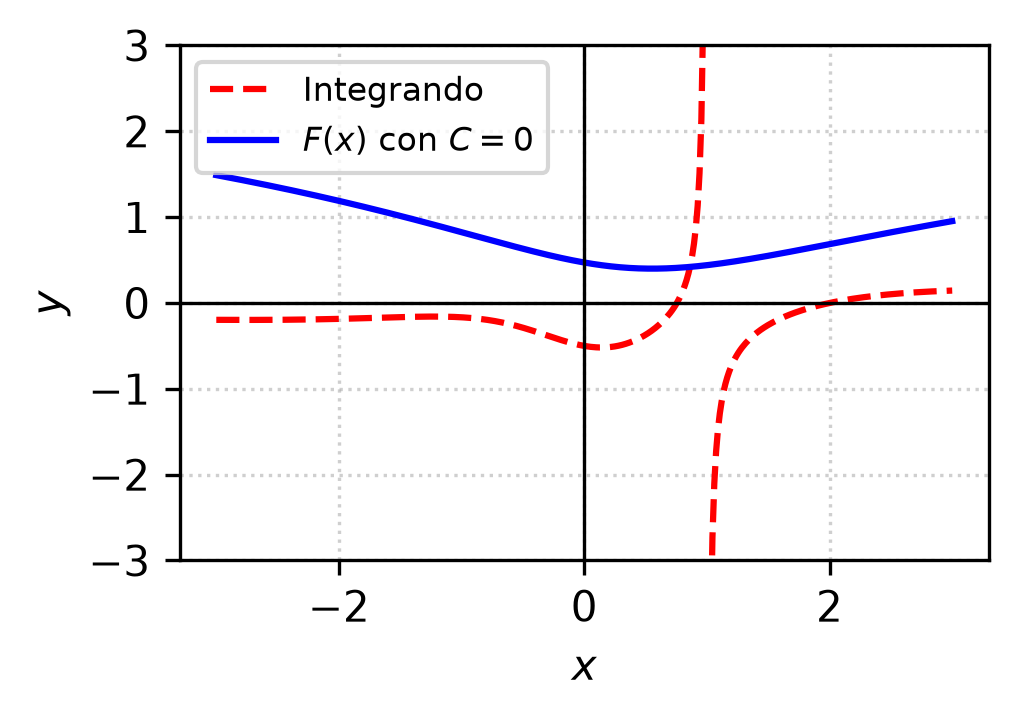
\includegraphics[width=\columnwidth]{semana_03/graficas/SEM03_P20_grafica.png}
	\caption{Representación gráfica de $f(x)$ y su antiderivada $F(x)$ evaluada para la constante de integración $C = 0$ (Problema 20).}
	\label{fig:problema20}
\end{figure}
